Interaction with computers can go far beyond typing on the keyboard,
moving the mouse, and touching the screen. 
Recent advances in computer vision technology can recognize 
hand gestures and body shape, as seen in Kinect games. 
With new computer vision devices such as the Leap Motion controller (), 
 precise 3D finger data can be obtained at over 100 frames per second.   
Therefore, it is possible to track the detailed positions of 
each finger precisely and efficiently. 
We advocate a new way to control computers by interpreting finger
movements as commands or character input using finger tracking devices.
In this paper, we propose a novel method to recognize handwritten
 characters in the air using such devices. 

\marginpar{
\begin{figure}
  \begin{center}
  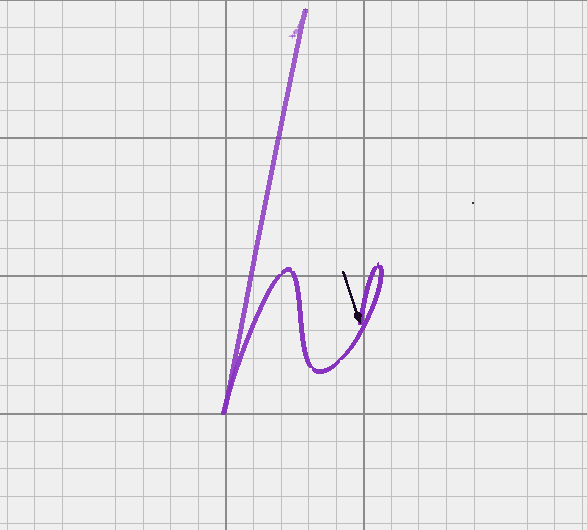
\includegraphics[width=1.75in]{images/he-2d-white-cropped.PNG}
  \caption{A 2D view of ``he'' sequence captured by Leap Motion controller.}
  \label{fig:he}
  \end{center}  
\end{figure}
}

Traditional character recognition technology is widely applied to such problems
as converting scanned books to text and converting images of bank checks into
valid payments. These problems can be divided into offline and online
recognition. 

We introduce a new problem: the online recognition of characters in a
 stream of 3D points from finger gestures. 
 Many OCR techniques utilize images of completed words, 
 whereas this paper deals with interpreting the data while it is generated,
specifically for the scenario of writing "in the air."  
In this paper we proposes a method of online character recognition, 
using a data-driven approach. 
Our method utilizes similarity search
technique on multi-dimensional time series. Figure~\ref{fig:he} shows a sample
sequences of 3D positions transformed from the tracked finger movement data. Our proposed approach to identify characters in these time series
 exploits the dynamic time warping (DTW) algorithm. 
A series of recent optimizations make a
DTW similarity search feasible in real time. This paper benchmarks the
performance of such a similarity search with the given application of
handwriting recognition.



The task of identifying characters in a time series requires data to test and
train on. Therefore, a new dataset needs to be created, partitioned into
 multiple candidate time series, specifically the characters in the alphabet,
  and multiple testing time series, which are words to be recognized. 
To construct this dataset, the Leap Motion, a commercial computer vision device,
is used to record data. The experiment will consist of collecting the same data
from over 100 people to account for differences in handwriting.

Our approach aims to deal with a less restricted kind of input than current
recognition techniques require. Related work shows that much of modern
handwriting recognition relies on a pen up/pen down gesture to 
The difference between our approach and other current handwriting recognition
approaches is the medium in which writing takes place. In many handwriting
recognition scenarios, the writing has already taken place and is being
statically analyzed. 
In our approach, we are dealing with live, free form input. 
Other related work shows the necessity of some pen up/pen down gesture 
to determine the beginning and end of meaningful input. 
Our approach attempts gives a less restricted form of input, 
where no strict gesture is necessary to identify meaningful data.

